% !TeX root = RJwrapper.tex
\title{\pkg{blindrecalc} - An R Package for Blinded Sample Size
Recalculation}
\author{by Lukas Baumann, Maximilian Pilz, and Meinhard Kieser}

\maketitle

\abstract{%
Besides the type 1 and type 2 error rate and the clinically relevant
effect size, the sample size of a clinical trial depends on so-called
nuisance parameters for which the concrete values are usually unknown
when a clinical trial is planned. When the uncertainty about the
magnitude of these parameters is high, an internal pilot study design
with a blinded sample size recalculation can be used to achieve the
target power even when the initially assumed value for the nuisance
parameter is wrong. In this paper, we present the R-package
\pkg{blindrecalc} that helps with planning a clinical trial with such a
design by computing the operating characteristics and the distribution
of the total sample size under different true values of the nuisance
parameter. We implemented methods for continuous and binary outcomes in
the superiority and the non-inferiority setting.
}

\hypertarget{introduction}{%
\section{Introduction}\label{introduction}}

Determining the sample size that is necessary to achieve a certain
target power is a fundamental step in the planning phase of every
clinical trial. The sample size depends on the type 1 error rate
\(\alpha\), the type 2 error rate \(\beta\), the effect size \(\Delta\)
and so-called nuisance parameters, which are parameters that affect the
distribution of the test statistic but are not of interest in the test
problem. While the type 1 and type 2 error rates are usually
predetermined and the minimal clinically important effect size is known,
there is often uncertainty about the magnitude of the nuisance
parameters, such as the variance of the data \(\sigma^2\) for tests with
continuous outcomes or the overall response rate \(p\) for tests with
binary outcomes.

Consider, as an example, the meta analysis by \citet{Nakata} that
compares minimally invasive preservation with splenectomy during distal
pancreatectomy. Among others, the overall morbidity of the two groups is
compared and data from 13 studies are reported (cf.~Figure 2(c) in
\citet{Nakata}). Within these 13 studies, overall morbidity rates pooled
over both groups between 0.10 and 0.62 are reported. This illustrates
the high uncertainty about the ``true'' overall morbidity rate, which is
the nuisance parameter in this setting.

In these cases, an internal pilot study design with blinded sample size
recalculation can be used. In such a design, the nuisance parameter is
estimated in a blinded way (i.e., without using information about the
group assignment of the patients) after a certain number of outcome data
is available, and the sample size is recalculated using this information
\citep{Wittes1990}. While in principle blinded sample size recalculation
could be done without any a priori sample size calculation, it is still
advisable to calculate an initial sample size based on the best guess
for the nuisance parameter available in the planning phase and to
determine when to recalculate the sample size based on this initial
calculation. This is done to avoid conducting the recalculation too
early (so that there is still a great uncertainty about the magnitude of
the nuisance parameter when recalculation is performed), or too late (so
that there may be no room for adjusting the sample size any longer as
the recalculated sample size is already exceeded). Using this method to
recalculate the sample size is an attractive option because the cost in
terms of additional sample size is very small (depending on the outcome)
and in most scenarios the type 1 error rate is unaffected by the blinded
sample size recalculation. Hence, whenever there is uncertainty about
the value of a nuisance parameter and the logistics of the trial allow
it, blinded sample size recalculation can be used. Meanwhile, this is
even recommended by regulatory authorities. For instance, the
\citet{CHMP} states that ``(w)henever possible, methods for blinded
sample size reassessment (\ldots) should be used''.

Methods to reassess the sample size in a blinded manner in an internal
pilot study design have been developed for a variety of outcomes. Based
on the early work by \citet{Stein}, \citet{Wittes1990} introduced the
internal pilot study design for continuous outcomes. Their work was
extended in different manners by different authors (cf.~among others
\citet{Birkett1994}, \citet{Denne1999}, and \citet{KF2000}). In all
these papers, the main task is to re-estimate the variance of a
continuous outcome in a blinded way. These ideas can be applied to
binary outcomes as well where the re-estimated nuisance parameter is the
overall response rate over both treatment arms. Associated methods were,
for instance, presented by \citet{Gould1992} and \citet{FK2004} for
superiority trials and by \citet{Friede2007} for non-inferiority trials.

However, despite the clear benefit of a blinded sample size
recalculation and a great number of publications on that topic,
\pkg{blindrecalc} is to the knowledge of the authors the first R-package
on CRAN, and thus a freely available software, that helps with the
planning of a clinical trial with such a design by computing the
operating characteristics and the distribution of the total sample size
of the study. The package can be used for pre-planned and midcourse
implemented blinded sample size reassessments in order to evaluate the
potential scenarios the blinded sample size re-estimation may imply. For
continuous outcomes, we implemented the \(t\)-test for superiority
trials and the shifted \(t\)-test for non-inferiority trials. For binary
outcomes, we implemented the chi-squared test for superiority trials and
the Farrington-Manning test for non-inferiority trials.

The structure of the paper is as follows: In the
\protect\hyperlink{statistical-methods}{Statistical methods} section, we
explain the general way of proceeding when conducting a trial with an
internal pilot study and how to obtain a blinded estimate of the
nuisance parameter for continuous and binary outcomes. The structure of
the package is introduced in
\protect\hyperlink{package-structure}{Package structure}. We demonstrate
how \pkg{blindrecalc} can be utilized to plan a trial with an internal
pilot study design and blinded sample size recalculation in
\protect\hyperlink{usage-and-example}{Usage and example}. In
\protect\hyperlink{development-principles}{Development principles}, we
outline the principles of the development process and how we ensure the
quality of our code. Finally, a brief
\protect\hyperlink{conclusion}{Conclusion} complements this paper.

\hypertarget{statistical-methods}{%
\section{Statistical methods}\label{statistical-methods}}

The general procedure for planning and conducting a trial with a blinded
sample size recalculation is as follows: At first, an initial sample
size \(n_{init}\) is calculated by using a best guess for the value of
the nuisance parameter. The sample size for the first stage of the
trial, \(n_1\), is then calculated as a fraction of \(n_{init}\), e.g.,
0.25, 0.5 or 0.75. After \(n_1\) observations are available, the total
sample size \(n_{rec}\) is recalculated in a blinded way based on the
available data. The final total sample size \(n\) is then determined as:
\[ n = \min\left(\max\left(n_1, n_{rec}\right), n_{max}\right),\] 
where \(n_{max}\) is a prespecified maximal sample size.
This is called the unrestricted design with upper boundary. 
A restricted design would use \(n_{init}\) as a
lower boundary \citep{Wittes1990}. Often \(n_{max}\) is set to a
multiple of \(n_{init}\). The special case of \(n_{max} = \infty\)
results in the unrestricted design \citep{Birkett1994}. After the final
total sample size is calculated, the \(n_2 = n - n_1\) observations for
the second stage are gathered. Finally, the specified statistical test
can be conducted with the data of all \(n\) patients.

In the following, we shortly introduce the implemented tests and how to
obtain a blinded estimate of the nuisance parameter in each case.

\hypertarget{continuous-outcomes}{%
\subsection{Continuous outcomes}\label{continuous-outcomes}}

Assume a clinical two-arm trial with normally distributed outcomes where
a higher value is deemed to be favorable, with mean values \(\mu_E\)
(experimental group) and \(\mu_C\) (control group) and common unknown
variance \(\sigma^2\). The outcome of interest is the mean difference
\(\Delta := \mu_E - \mu_C\). By introducing a non-inferiority margin
\(\delta>0\), the test problem is given by
\[H_0: \Delta \leq - \delta \text{ vs. } H_1: \Delta > -\delta.\] The
null hypotheses can be tested by a shifted \(t\)-test taking the
non-inferiority margin \(\delta\) into account. Note that the special
case \(\delta=0\) corresponds to the standard \(t\)-test for
superiority. The approximate total sample size for a one-sided
\(t\)-test to detect a mean difference of
\(\Delta = \Delta^* > -\delta\) with a power of \(1-\beta\) while
controlling the type 1 error rate at level \(\alpha\) equals
\[n=n_E+n_C=\frac{\left(1+r\right)^2}{r} \frac{\left(z_{1-\alpha/2} + z_{1-\beta}\right)^2 \sigma^2}{\left(\Delta^*+\delta\right)^2}.\]
Here, \(r\) refers to the allocation ratio of the sample sizes between
the experimental and the control group, i.e., \(r = n_E / n_C\), and
\(z_{1-q}\) denotes the \(1-q\) quantile of the standard normal
distribution.

In this framework, the nuisance parameter is the unknown variance
\(\sigma^2\). Due to potential uncertainty on the value of \(\sigma^2\),
it seems appropriate to re-estimate it in a blinded interim analysis to
ensure that the desired power level is met. Inserting
\(\widehat{\sigma}^2\) observed mid-course into the above sample size
formula may lead to a more reasonable sample size for the respective
trial than sticking to the value assumed in the planning stage. There
exist different methods for estimating \(\sigma^2\) in a blinded manner
\citep{Zucker1999}. In \pkg{blindrecalc}, the one-sample variance
estimator is implemented. It is defined as \[
\widehat{\sigma}^2 := \frac{1}{n_1-1} \sum_{j \in \{E, C \}} \sum_{k=1}^{n_{1,j}}
\left( x_{j,k} - \bar{x} \right)^2,
\] where \(x_{j,k}\) is the outcome of patient \(k\) in group \(j\),
\(n_{1,j}\) denotes the first-stage sample size in group \(j\), i.e.,
\(n_1 = n_{1,E} + n_{1,C}\), and \(\bar{x}\) equals the mean over all
\(n_1\) observations. Since the patient's group allocation is not
considered when computing \(\widehat{\sigma}^2\), blinding is maintained
when using this variance estimator.

In the superiority case, i.e., if \(\delta=0\), blinded sample size
reassessment can be performed without relevant type 1 error rate
inflation \citep{KF2003}. In the non-inferiority case, however, the type
1 error rate may be inflated by the internal pilot study design and a
correction of the applied significance level may become necessary to
protect the nominal type 1 error rate at level \(\alpha\)
\citep{FK2003}. In particular, this inflation arises if the sample size
recalculation is performed too early, i.e., if \(n_1\) is chosen too
small.

Interestingly, the cost of this procedure in terms of sample size is
quite low. Since the one-sample variance estimate slightly overestimates
the variance, an increase in sample size arises. However, this increase
amounts to only 8 patients with \(\alpha = 0.025\) and \(\beta = 0.2\)
or 12 patients with the same significance level and \(\beta = 0.1\)
\citep{FK2001}. In return, the sample size recalculation procedure
implies that the trial's power meets the target value \(1-\beta\) for a
wide range of values of \(\sigma^2\).

\citet{Lu2016} gives closed formulas for the exact distribution of the
test statistic of the two-sample \(t\)-test in this setting. This allows
the simulation of error probabilities and of the sample size
distribution in an acceptable amount of time. The proposals made by
\citet{Lu2016} are implemented in \pkg{blindrecalc}. Thus, the design
characteristics for continuous outcomes presented in \pkg{blindrecalc}
are obtained by simulation and not by exact computation. This is the
case for for binary outcomes that are presented in the following.

\hypertarget{binary-outcomes}{%
\subsection{Binary outcomes}\label{binary-outcomes}}

In a superiority trial with binary outcomes where a higher response
probability is assumed to be favorable, the one-sided null and
alternative hypothesis are
\[H_0: p_E \leq p_C \text{ vs. } H_1: p_E > p_C,\] where \(p_E\) and
\(p_C\) denote the event probabilities in the experimental and the
control group, respectively. While several tests exist for this test
problem, the widely used chi-squared test is implemented in
\pkg{blindrecalc}. The sample size for this test can be approximated
with the formula \citep{Kieser2020}:
\[n = \frac{1 + r}{r} \frac{\left(z_{1 - \alpha / 2} 
\sqrt{\left(1 + r\right) \cdot p_0 \cdot \left(1 - p_0\right)} + z_{1 - \beta} 
\sqrt{r \cdot p_{C,A} \cdot \left(1 - p_{C,A}\right) + 
p_{E,A} \cdot \left(1 - p_{E,A}\right)}\right)^2}
{\Delta^2}.\] Again, \(r\) denotes to the allocation ratio of the sample
sizes, and \(z_{1 - \alpha / 2}\) and \(z_{1 - \beta}\) are the
\(1 - \alpha / 2\) and the \(1 - \beta\) quantiles of the standard
normal distribution. Furthermore, \(p_{C,A}\) and \(p_{E,A}\) are the
response probabilities in the control and the experimental group under
the assumed alternative, \(p_0\) is the overall response probability,
i.e., \(p_0 = \left(p_{C,A} + r \cdot p_{E,A}\right) / \left(1 + r\right)\), and \(\Delta\) is
the effect under the alternative, i.e.~\(\Delta = p_{E,A} - p_{C,A}\).
The nuisance parameter here is \(p_0\), which can be estimated in a
blinded way after \(n_1\) observations with
\[\hat{p}_0 = \frac{X_{1,E} + X_{1,C}}{n_{1,E} + n_{1,C}},\] where
\(X_{1,E}\) and \(X_{2,C}\) denote the number of observed events in the
experimental and the control group and \(n_{1,E}\) and \(n_{1,C}\)
represent the first-stage sample sizes in the two groups. Blinded
estimates of the event rates in each group can then be obtained by
\(\hat{p}_{C,A} = \hat{p}_0 - \Delta \cdot r / \left( 1 + r \right)\) and
\(\hat{p}_{E,A} = \hat{p}_0 + \Delta / \left(1 + r\right)\). These estimates are
used to recalculate the sample size. The benefit of the blinded
recalculation is that the desired power can be maintained, even if the
initially assumed value for \(p_0\) was wrong.

It is well known that the chi-squared test in a fixed design does not
maintain the nominal significance level, hence the same can be expected
for a chi-squared test with a blinded sample size recalculation. In
fact, \citet{FK2004} showed that the actual levels of the test with and
without recalculating the sample size are very close.

In a non-inferiority trial, the null and alternative hypothesis are
\[H_0: p_E - p_C \leq - \delta \text{, } H_1: p_E - p_C > -\delta,\]
where \(\delta > 0\) is the fixed non-inferiority margin. The most
commonly used test for this problem was proposed by \citet{FM1990}.
An approximate sample size formula for this test is
\[n = \frac{1 + r}{r} \cdot \frac{\left(z_{1 - \alpha / 2} 
\sqrt{r \cdot \tilde{p}_C \cdot \left(1 - \tilde{p}_C\right) + 
\tilde{p}_E \cdot \left(1 - \tilde{p}_E \right)} + z_{1 - \beta}
\sqrt{r \cdot p_{C,A} \cdot \left(1 - p_{C,A}\right) + 
p_{E,A} \cdot \left(1 - p_{E,A}\right)} \right)^2}{\left(\Delta + \delta\right)^2},\] where
\(\tilde{p}_{E}\) and \(\tilde{p}_{C}\) are large sample approximations
of the restricted maximum likelihood estimators under the null
hypothesis restriction \(p_E - p_c = - \delta\) (see the Appendix of
\citet{FM1990} for the computation). The same formulas as for the
chi-squared test can be used to estimate \(\hat{p}_E\) and \(\hat{p}_C\)
in a blinded way, and these estimates have to be used to obtain blinded
estimates \(\hat{\tilde{p}}_E\) and \(\hat{\tilde{p}}_C\) for the
restricted maximum likelihood estimates. Plugging these estimates into
the sample size formula gives the re-estimated sample size.

Like the chi-squared test, the Farrington-Manning test is also no exact
test and can exceed the nominal significance level. \citet{Friede2007}
showed that in general no further inflation of the type 1 error rate is
caused by blinded re-estimation of the sample size. Nevertheless, it is
possible for the chi-squared test as well as for the Farrington-Manning
test to choose the nominal significance level smaller than \(\alpha\) in
order to protect the type 1 error rate at level \(\alpha\). Such an
adjustment of \(\alpha\) is implemented in \pkg{blindrecalc} for the
binary and the continuous case.

\hypertarget{package-structure}{%
\section{Package structure}\label{package-structure}}

When a clinical trial with an internal pilot study is planned, it is
essential to know the characteristics of the applied design. To this
end, the performance in terms of achieved power levels, type I error
rates, and sample size distribution has to be known for different values
of the nuisance parameter and the first-stage sample size \(n_1\). The
package \pkg{blindrecalc} provides all necessary tools that are needed
to plan a trial with a blinded sample size recalculation with only a
small number of functions, which makes using the package very
accessible.

\pkg{blindrecalc} makes use of R's S4 class system. This allows the
application of the same methods for different design classes and
facilitates the usage of the package. Furthermore, this approach makes
the package easily extendable without any changes in the current source
code.

The usage of \pkg{blindrecalc} is intended to be as intuitive as
possible. To obtain characteristics of a blinded sample size
recalculation procedure, two steps have to be made. At first, the user
has to define a design object to indicate which test and which
characteristics such as the desired type 1 and type 2 error rates are to
be applied. To this end, the three functions \code{setupChiSquare},
\code{setupFarringtonManning}, and \code{setupStudent} exist to define a
design object of the class corresponding to the respective test.

Secondly, the trial characteristic of interest can be calculated.
Currently, the following methods are implemented: The method \code{toer}
allows the computation of the actual type 1 error rate for different
values of the nuisance parameter and the sample size of the internal
pilot study. By means of \code{adjusted\_alpha}, the adjusted
significance level can be calculated that can be applied as nominal
significance level when strict type 1 error rate control is desired. The
method \code{pow} computes the achieved power of the design under a
given set of nuisance parameters or internal pilot sample sizes. With
\code{n\_fix}, the sample size of the corresponding fixed design can be
computed. Finally, the method \code{n\_dist} provides plots and
summaries of the distribution of the sample size. For all these methods
(except for \code{n\_dist}), the logical parameter \code{recalculation}
allows to define whether a fixed design or a design with blinded sample
size recalculation is analyzed.

\hypertarget{usage-and-example}{%
\section{Usage and example}\label{usage-and-example}}

For each test, there is a \code{setup} function (e.g.,
\code{setupChiSquare} for the chi-squared test) that creates an object
of the class of the test. Each \code{setup} function takes the same
arguments:

\begin{itemize}
\tightlist
\item
  \code{alpha}: The one-sided type 1 error rate.
\item
  \code{beta}: The type 2 error rate.
\item
  \code{r}: The allocation ratio between experimental and control group,
  with a default of 1.
\item
  \code{delta}: The difference in effect size between alternative and
  null hypothesis.
\item
  \code{alternative}: Whether the alternative hypothesis contains
  greater (default) or smaller values than the null.
\item
  \code{n\_max}: The maximal total sample size, with a default value of
  \code{Inf}.
\end{itemize}

In this example, the nuisance parameter is the overall response rate
\(p\). A difference in response rates between the two treatment groups
of \(\Delta = p_{E} - p_{C} = 0.2\) is to be detected. Using
\pkg{blindrecalc}, a chi-squared test that achieves a power of
\(1 - \beta = 0.8\) to detect this effect of \(\Delta = 0.2\) and that
uses a nominal type 1 error rate of \(\alpha = 0.025\) can be set up by

\begin{example}
design <- setupChiSquare(alpha = 0.025, beta = 0.2, delta = 0.2)
\end{example}

The sample size for a fixed design given one or multiple values of the
nuisance parameter (argument \code{nuisance}) can then be calculated
with the function \code{n\_fix}:

\begin{example}
n_fix(design, nuisance = c(0.2, 0.3, 0.4, 0.5))
#> [1] 124 164 186 194
\end{example}

The function \code{toer} calculates the actual level of a design with
blinded sample size recalculation or of a fixed design (logical argument
\code{recalculation}) given either one or more values of the total
sample size in a fixed or the sample size for the first stage in a
recalculation design (argument \code{n1}) or one or more values of the
nuisance parameter. Note that all functions are only vectorized in one
of the two arguments \code{n1} and \code{nuisance}. In this example, it
is assumed that the internal pilot study contains half of the fixed
sample size that would be needed if the overall response rate \(p\)
equals \(0.2\). In this setting, \pkg{blindrecalc} can be used to
compare the actual levels of a fixed design and a recalculation design
with the same parameters.

\begin{example}
n <- n_fix(design, nuisance = 0.2)
p <- seq(0.1, 0.9, by = 0.01)
toer_fix <- toer(design, n1 = n, nuisance = p, recalculation = FALSE)
toer_ips <- toer(design, n1 = n/2, nuisance = p, recalculation = TRUE)
\end{example}

In Figure \ref{fig:toer}, the type 1 error rate in dependence of the
nuisance parameter is depicted for the designs with and without sample
size recalculation. Note that, as mentioned in Section
\protect\hyperlink{binary-outcomes}{Binary outcomes}, the level of
significance exceeds the pre-defined level of \(\alpha = 0.025\) in both
cases. If strict control of the type 1 error rate is desired, the
function \code{adjusted\_alpha} can be used to to calculate an adjusted
significance level, such that the nominal significance level is
preserved.

\begin{example}
adj_sig <- adjusted_alpha(design, n1 = n/2, nuisance = p, precision = 0.0001,
                          recalculation = TRUE)
design@alpha <- adj_sig
toer_adj <- toer(design, n1 = n/2, nuisance = p, recalculation = TRUE)
\end{example}

In this example, the adjusted significance level equals 0.0232 for the
trial with internal pilot study, i.e., using this value as nominal level
ensures that the actual significance level does not exceed
\(\alpha = 0.025\). Figure \ref{fig:toer} demonstrates that the type 1
error rate is protected at level \(\alpha = 0.025\) if the adjusted
significance level is applied.

In the setting of binary outcomes, adjusting the level such that the
nominal type 1 error rate is protected for any realization of the
nuisance parameter in its domain \([0, 1]\) is feasible. However, when
the nuisance parameter has an infinite domain, such as the variance in
the case of continuous outcomes, this is not possible. The solution in
these cases is to compute a \(\left(1 - \gamma\right)\) confidence interval of
the nuisance parameter in the blinded interim analysis and adjust the
significance level such that the actual level is below
\(\alpha - \gamma\) for all values in this confidence interval
\citep{FK2011}. If this approach is applied, the user can set the
parameter \code{gamma}.

\begin{figure}
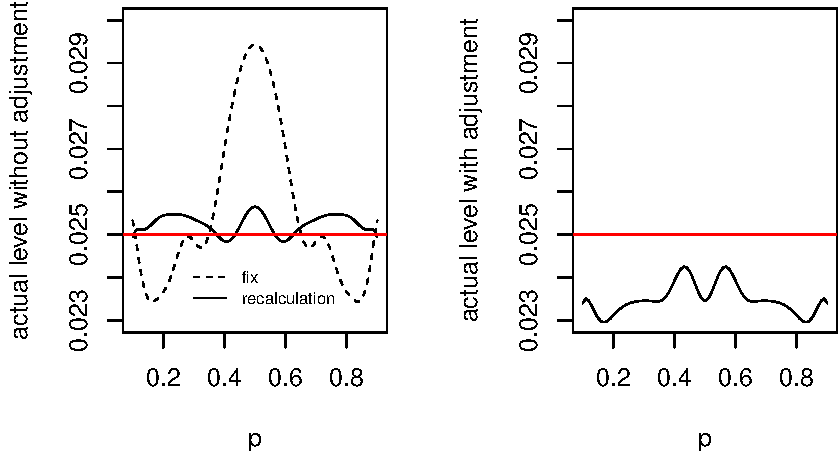
\includegraphics{blindrecalc_paper_files/figure-latex/plot-type-1-error-1} \caption{\label{fig:toer}Actual significance level for different nuisance parameters with (right panel) and without (left panel) adjustment of the nominal significance level. In the adjusted case, the actual level is below the desired level (red line) for all nuisance parameters in contrast to the un-adjusted case.}\label{fig:plot-type-1-error}
\end{figure}

To calculate the power of either the internal pilot study design or the
fixed design, the function \code{pow} can be used. Again, the function
is vectorized in either \code{n1} or \code{nuisance}. This function can
be used to compare the power values of the two designs under different
actual values of the nuisance parameter.

\begin{example}
pow_fix <- pow(design, n1 = n, nuisance = p, recalculation = FALSE)
pow_ips <- pow(design, n1 = n/2, nuisance = p, recalculation = TRUE)
\end{example}

\begin{figure}
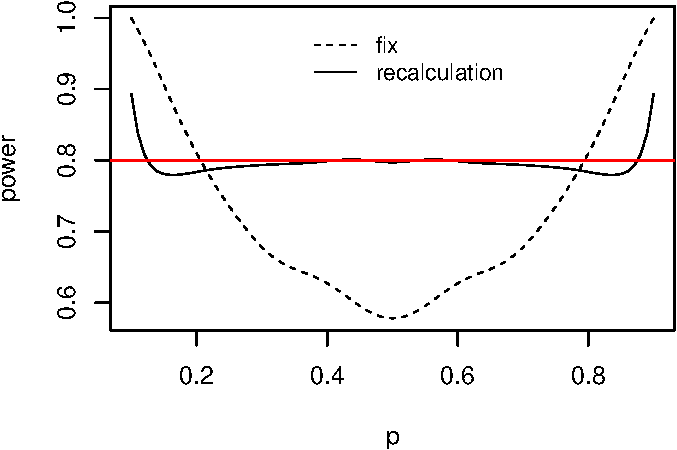
\includegraphics{blindrecalc_paper_files/figure-latex/plot-power-1} \caption{\label{fig:pow}Power values for different nuisance parameters for a fixed design and a design with blinded sample size recalculation. The design with recalculation meets the target power (red line) for a wider range of nuisance parameters.}\label{fig:plot-power}
\end{figure}

As we can see in Figure \ref{fig:pow}, the power achieved by the
internal pilot study design is very close to the target power of 0.8 in
most cases. Only when the overall response rate is very close to 0 or 1,
the power is exceeded. On the other hand, the fixed design is much more
sensitive to the actual value of the nuisance parameter and the actual
power can either be way too large or way too small if the sample size
was calculated under wrong assumptions.

Finally, the distribution of the total sample size can be computed under
different assumptions on the nuisance parameter with the function
\code{n\_dist}. This is particularly useful for the planning of internal
pilot study designs since it allows the investigation of what could
happen in a certain clinical trial and helps the applicant to prepare
for different scenarios.

\begin{example}
p <- seq(0.2, 0.8, by = 0.1)
n_dist(design, n1 = n/2, nuisance = p, plot = TRUE)
\end{example}

\begin{figure}
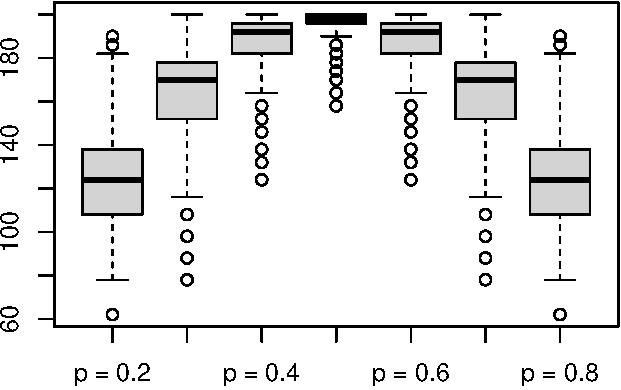
\includegraphics{blindrecalc_paper_files/figure-latex/sample-size-distribution-1} \caption{\label{fig:dist}Distribution of the sample size for a design with blinded sample size recalculation in dependence of the nuisance parameter. For more extreme values of the nuisance parameter the variance of the sample size distribution becomes larger.}\label{fig:sample-size-distribution}
\end{figure}

\begin{example}
#>         p = 0.2  p = 0.3  p = 0.4  p = 0.5  p = 0.6  p = 0.7 p = 0.8
#> Min.     62.000  78.0000 124.0000 158.0000 124.0000  78.0000  62.000
#> 1st Qu. 108.000 152.0000 182.0000 196.0000 182.0000 152.0000 108.000
#> Median  124.000 170.0000 192.0000 198.0000 192.0000 170.0000 124.000
#> Mean    125.021 164.6057 188.4801 196.5075 188.4801 164.6057 125.021
#> 3rd Qu. 138.000 178.0000 196.0000 200.0000 196.0000 178.0000 138.000
#> Max.    190.000 200.0000 200.0000 200.0000 200.0000 200.0000 190.000
\end{example}

By default, \code{n\_dist} prints a summary of the sample size
distribution for each nuisance parameter. With \code{plot = TRUE}, a
series of boxplots is drawn (cf.~Figure \ref{fig:dist}). Since the
maximum sample size is obtained if the overall response rate is
estimated to be 0.5 in the sample size recalculation, this maximum can
occur under any true value of the nuisance parameter (except for 0 and
1), albeit with very small probability. For this reason, sample sizes
that occur with a probability of less than 0.01\% are ignored. This is
not the case for continuous outcomes since there, the sample size
distributions are determined by simulation.

For continuous outcomes, i.e., the (shifted) \(t\)-test, the functional
content of \pkg{blindrecalc} is the same as in the binary case that was
presented in this example. The only difference is that in the continuous
case, the numbers are computed by simulation. Thus, the user can set the
parameters \code{iters}, defining the number of simulation iterations,
and \code{seed}, the random seed for the simulation.

\hypertarget{development-principles}{%
\section{Development principles}\label{development-principles}}

The utilization of R's object-oriented programming capabilities implies
that the example that was presented for the chi-squared test could very
similarly be applied to the Farrington-Manning test or the \(t\)-test.
Besides using S4 classes, the following development principles of
\pkg{blindrecalc} should be briefly described.

All calculations for binary outcomes are exact and require nested
for-loops. Since for-loops are known to be very slow in R, all
computation-intensive functions for the chi-squared test and the
Farrington-Manning test are implemented in C++ via the \CRANpkg{Rcpp}
package \citep{Rcpp} to speed up the calculations significantly.

\pkg{blindrecalc} is developed open-source on GitHub.com. The entire
source code can be found at
\url{https://github.com/imbi-heidelberg/blindrecalc}. This allows anyone
to contribute to \pkg{blindrecalc} and, furthermore, provides maximal
transparency. To ensure a certain quality of the provided code,
\pkg{blindrecalc} is checked by unit tests using the package
\CRANpkg{covr} \citep{covr}. The unit tests compare numbers for the
sample size, type 1 error rate, and power calculated with
\pkg{blindrecalc} with numbers from peer-reviewed publications and,
furthermore, check the technical functionality of the package such as
vectorization and display of error messages. Thus, the unit tests do not
only monitor the technical accuracy of the package's results but also
their content-related correctness. The current version \pkg{blindrecalc}
0.1.3 achieves a code coverage of 100\%, i.e., each line of the source
code is checked by at least one unit test.

\hypertarget{conclusion}{%
\section{Conclusion}\label{conclusion}}

In this paper, we introduced the R-package \pkg{blindrecalc} that can be
used to plan clinical trials with a blinded sample size recalculation in
an internal pilot study design when either continuous or binary outcomes
in a superiority or non-inferiority setting are of interest. We
introduced the basic methodology of internal pilot studies and explained
how the package can be used to calculate the operating characteristics
of a trial with such a design.

The scope of \pkg{blindrecalc} can simply be extended due to its modular
character. Blinded sample size recalculation can be applied to many
different types of clinical trials. For instance, there exists research
on further kinds of outcomes (e.g., see \citet{Friede2010} for count
data) or on different study designs (e.g., see \citet{Golkowski2014} for
bioequivalence trials). The implementation of internal pilot studies for
such cases in \pkg{blindrecalc} is an exciting area of future work.

\bibliography{blindrecalc-paper}

\hypertarget{contribution}{%
\section{Contribution}\label{contribution}}

The first two authors contributed equally to this manuscript.


\address{%
Lukas Baumann\\
Institute of Medical Biometry\\%
University of Heidelberg\\ Im Neuenheimer Feld 130.3\\ 69120
Heidelberg\\ Germany\\ ORCiD 0000-0001-7931-7470\\
%
%
%
\href{mailto:baumann@imbi.uni-heidelberg.de}{\nolinkurl{baumann@imbi.uni-heidelberg.de}}%
}

\address{%
Maximilian Pilz\\
Institute of Medical Biometry\\%
University of Heidelberg\\ Im Neuenheimer Feld 130.3\\ 69120
Heidelberg\\ Germany\\ ORCiD 0000-0002-9685-1613\\
%
%
%
\href{mailto:pilz@imbi.uni-heidelberg.de}{\nolinkurl{pilz@imbi.uni-heidelberg.de}}%
}

\address{%
Meinhard Kieser\\
Institute of Medical Biometry\\%
University of Heidelberg\\ Im Neuenheimer Feld 130.3\\ 69120
Heidelberg\\ Germany\\ ORCiD 0000-0003-2402-4333\\
%
%
%
\href{mailto:kieser@imbi.uni-heidelberg.de}{\nolinkurl{kieser@imbi.uni-heidelberg.de}}%
}
